\documentclass[10pt]{article}
\usepackage[margin=0.25in,footskip=0.10in]{geometry}
\usepackage{graphicx}
\usepackage{subfig}
\usepackage{alphalph}
\renewcommand*{\thesubfigure}{\arabic{subfigure}}
\usepackage{amsmath}
\usepackage{mathtools}
\usepackage{enumitem}
\usepackage{csquotes}
\usepackage{amssymb}
\usepackage{amsthm}
\usepackage{xcolor}
%\pagecolor[rgb]{0.0,0.0,0.0}
%\color[rgb]{1,1,1}
\title{Gray Immunity model - Summary of results}
\author{Himanshu A Bhisikar}
\date{}
\begin{document}
  \graphicspath{ {/home/maverick/IISER/'Milind Sir'/'Results'/'Results2'/} }
  \maketitle
  \section{Summary}
  \begin{itemize}
    \item We obtained 4 different types of curves in our model simulations -
    \begin{center}
      \begin{figure}[ht]
        \begin{tabular}{cc}
          \subfloat[\(0.2, 50\) - Multiple waves]{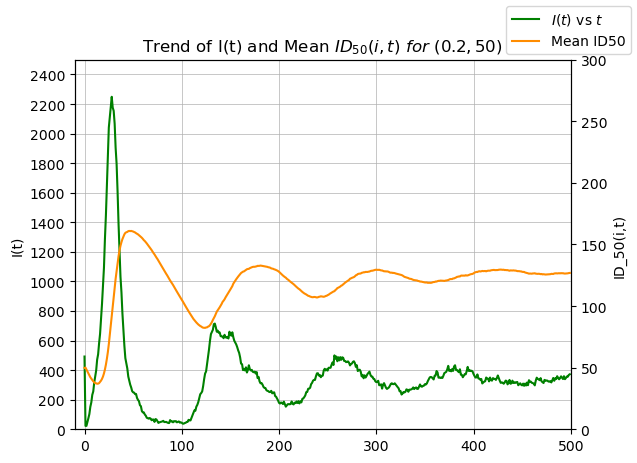
\includegraphics[width = 2.0in]{1-02-50.png}} &
          \subfloat[\(0.0, 50\) - Perfect control leading to extinction]{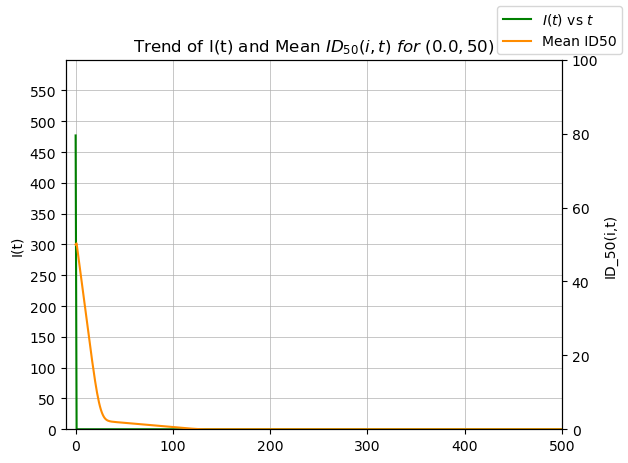
\includegraphics[width = 2.0in]{2-00-50.png}} \\
          \subfloat[\(0.6, 50\) - Single wave followed by Endemicity]{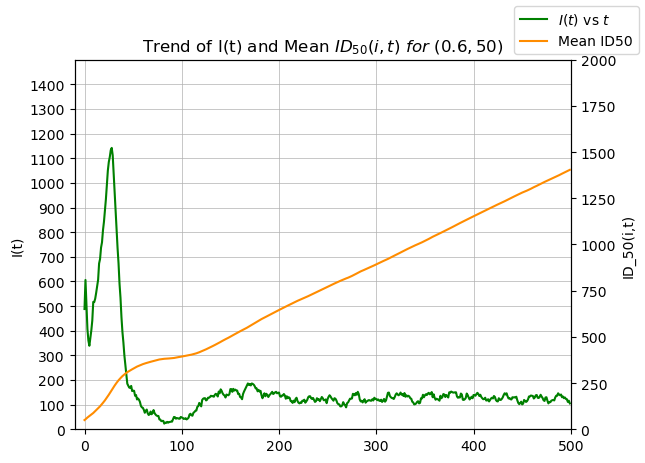
\includegraphics[width = 2.0in]{3-06-50.png}} &
          \subfloat[\(1.0, 20\) - Single wave followed by Extinction]{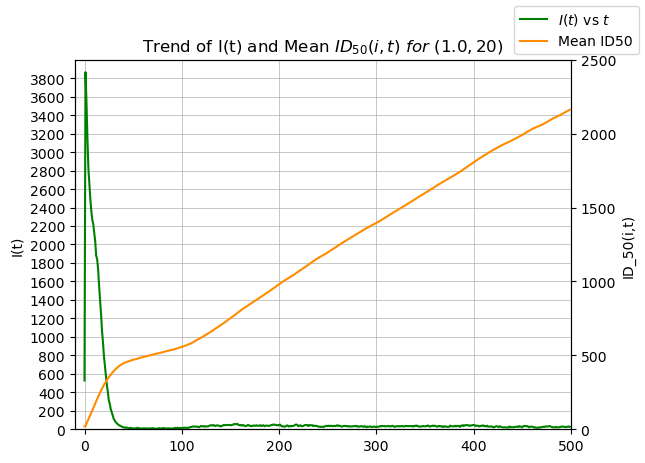
\includegraphics[width = 2.0in]{4-10-20.png}} \\
        \end{tabular}
      \end{figure}
    \end{center}
    \item The variation of mean \(ID_{50}\) values with changes in Cross-immunity parameter are shown in the corresponding 2 histograms -
    \begin{center}
      \begin{figure}[ht]
        \begin{tabular}{cc}
          \subfloat[\(0.0,20\)]{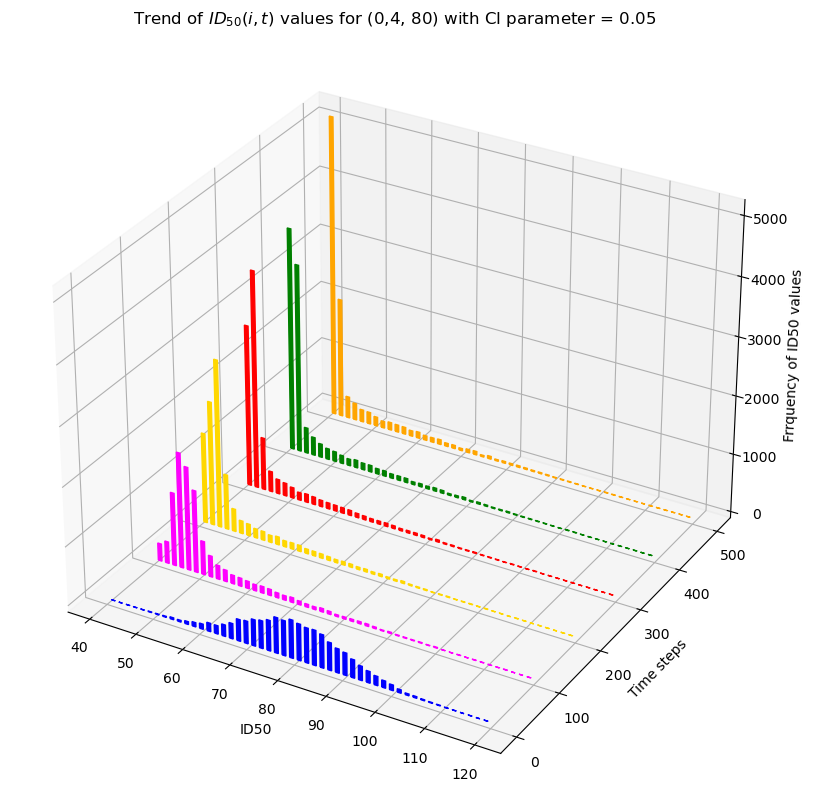
\includegraphics[width = 2.0in]{Cross_Immunity_(0,4,80)_0.05.png}} &
          \subfloat[\(0.2,20\)]{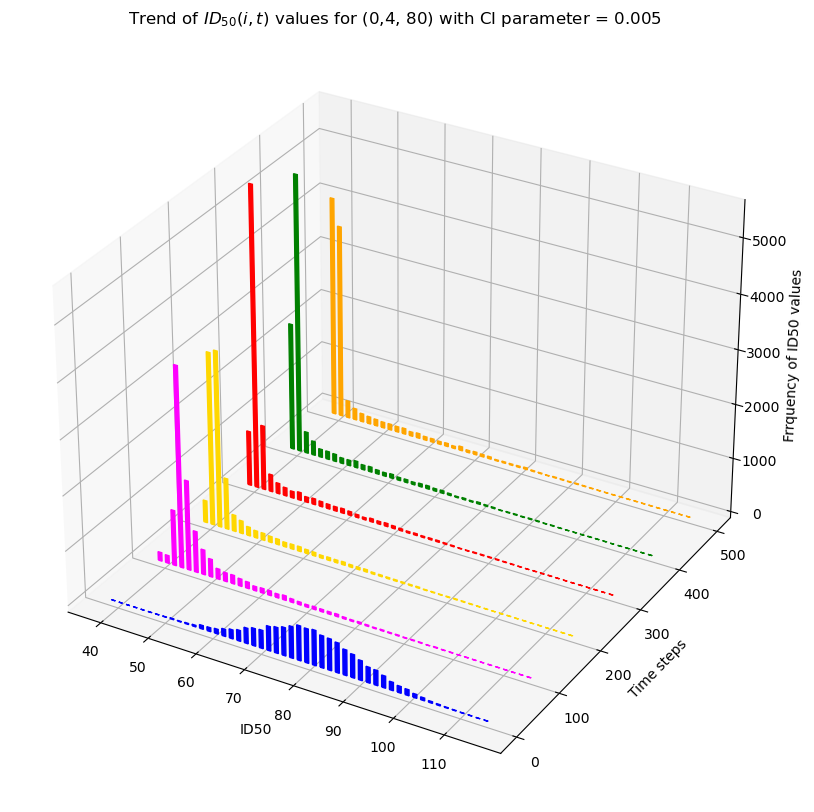
\includegraphics[width = 2.0in]{Cross_Immunity_(0,4,80)_0.005.png}} \\
        \end{tabular}
      \end{figure}
    \end{center}
  \end{itemize}
\end{document}
